% !TEX encoding = UTF-8
% !TEX TS-program = pdflatex
% !TEX root = ../tesi.tex

%**************************************************************
\chapter{Introduzione}
\label{cap:introduzione}
%**************************************************************
\section{Il progetto}
Zucchetti è un’azienda italiana che produce soluzioni software, hardware e servizi
per aziende, banche, assicurazioni, professionisti e associazioni di categoria. 
La sede principale è a Lodi, ma è ben radicata nel territorio nazionale e ha sedi sparse in tutto il mondo;
la sede padovana, in particolare, si occupa di ricerca e sviluppo.

Al momento Zucchetti può vantare una rete distributiva di oltre 1000 Partner, 130.000
clienti e più di 5500 addetti. Queste cifre proiettano il gruppo Zucchetti tra le aziende italiane 
più importanti nel settore dell’Information and Communications Technology(ICT) e come prima
software house italiana.

Con questi numeri è evidente che la formazione giochi un ruolo importante: a tal fine, infatti, la 
Zucchetti organizza corsi e dispone di un ampio catalogo di video formativi, di cui viene automaticamente 
estratta ed indicizzata la trascrizione dell’audio, per permettere un recupero puntuale dei filmati.

Il progetto di stage nasce dalla necessità di cercare di migliorare il recupero delle informazioni 
dal \gls{corpus}: una informazione che non si riesce a reperire è una informazione persa.

Lo stage ha comportato quindi lo studio di metodi per migliorare la precisione e il recupero delle informazioni
all’interno del corpus generato: era infatti evidente, da precedenti prove fatte in azienda, che il corpus
a disposizione non fosse sufficiente per permettere l’applicazione di 
metodi basati sul deeplearning come in particolare word2vec e le reti neurali associate e da qui la necessità di provare soluzioni alternative.

Durante queste otto settimane, i prodotti attesi erano:
\begin{enumerate}
    \item una pagina di ricerca per ogni metodo implementato; 
    \item una collezione di test;
    \item la documentazione del codice prodotto.
\end{enumerate}

Il progetto ha avuto inizio il 23 settembre 2019 ed è terminato il 16 novembre 2019, per
un totale di 320 ore.


%Introduzione al contesto applicativo.\\
%
%\noindent Esempio di utilizzo di un termine nel glossario \\
%\gls{api}. \\
%
%\cite{site:agile-manifesto}. \\
%
%\noindent Esempio di citazione nel pie' di pagina \\
%citazione\footcite{womak:lean-thinking} \\

%**************************************************************
\section{Strumenti utilizzati}
Come ambiente di lavoro, ho utilizzato il PC fornitomi dall'azienda e
quindi ho sviluppato principalmente su Windows 10.
Nella scelta degli strumenti da utilizzare è stata lasciata da parte dell'azienda
ampia libertà.

\begin{description}
    \item[Visual Studio Code] È stato scelto in quanto multipiattaforma e per 
    l'elevata possibilità di personalizzazione permesso dai plugin installati 
    nel market. Si è rivelato essere molto adatto alle mie esigenze:
    \begin{itemize}
        \item il plugin per il \gls{wsl}, che mi ha permesso di aggirare una limitazione nel redirect degli output della PowerShell di Windows ed eseguire lo script nella bash, senza dover uscire dal mio ambiente di lavoro; 
        \item le funzionalità di autocompletamento e Syntax highlighting hanno ridotto la possibilità di introdurre typo;
        \item il code formatter Prettier ha mantenuto il mio codice sempre ben formattato e quindi più leggibile.
    \end{itemize}
    
    \item[\gls{git}] per il versionamento del codice.
\end{description}

%**************************************************************
\section{Prodotto ottenuto}
\begin{center}
    \begin{figure}
        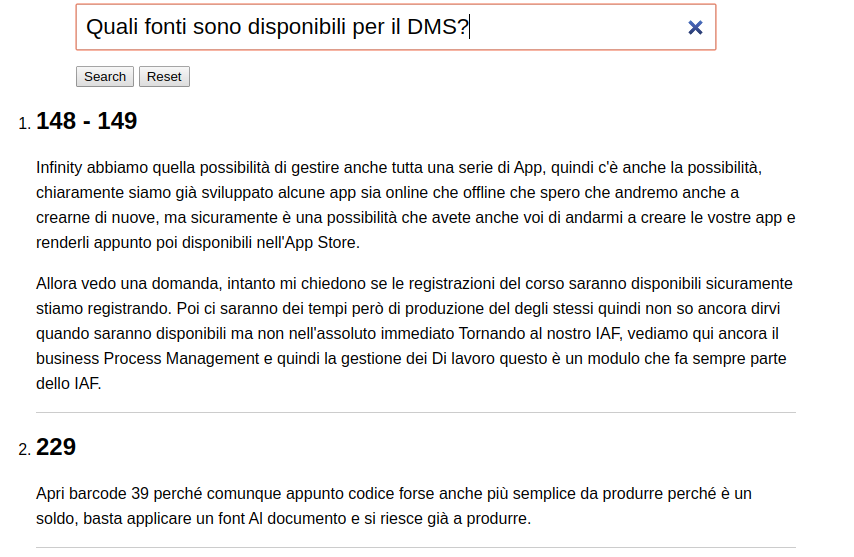
\includegraphics[scale=0.55]{immagini/ricerca.png}
        \caption{Esempio implementazione della ricerca}
     \end{figure}
\end{center}

È possibile effettuare una ricerca all'interno del corpus utilizzando un tesauro (manuale, generico o automaticamente generato) e l'analisi della semantica latente. È stato configurato uno stemmer italiano, basato sullo stemmer Snowball.

%**************************************************************
\section{Le principali problematiche}
\label{sec:problematiche}
Le principali difficoltà del progetto sono state derivanti da tre fattori:
\begin{enumerate}
    \item Difficoltà nel muovere i primi passi con la libreria lunr.js. Causa di questo problema è stata principalmente una limitata conoscenza da parte mia del linguaggio di programmazione Javascript: tale problema è stato risolto grazie allo studio individuale del linguaggio.
    \item Difficoltà nel stabilire quali documenti fossero pertinenti o meno rispetto a una ricerca. Questo problema deriva dagli errori introdotti dalla trascrizione automatica, rendendo inizialmente impossibile realizzare la ground truth richiesta. Il problema è stato superato una volta avuto accesso ai filmati e non solo alle trascrizioni.
    \item Difficoltà intrinseca del problema: riuscire ad ottenere dei buoni risultati con un corpus piccolo è intrinsecamente difficile: alcune strade possibili con un corpus grande non lo sono con uno piccolo (non solo i metodi basati sul deeplearning) e gli errori introdotti dalla trascrizione incidono molto di più di quanto non farebbero con un corpus grande. 
    \item Nessuna conoscenza pregressa del dominio. Prima dello stage, non ne sapevo nulla di recupero dell'informazione e alcuni argomenti all'inizio si sono rivelati essere un po' ostici: questo è stato risolto grazie allo studio individuale e l'aiuto da parte del mio tutor aziendale. 
\end{enumerate}

%**************************************************************
\section{Organizzazione del testo}

\begin{description}
    \item[{\hyperref[cap:analisi-requisiti]{Il secondo capitolo}}] descrive brevemente qual è il problema che bisognava affrontare ed elenca i requisiti individuati.
    
    \item[{\hyperref[cap:recupero-informazione]{Il terzo capitolo}}] introduce i concetti essenziali riguardanti il recupero dell'informazione.
    
    \item[{\hyperref[cap:latent-semantic-indexing]{Il quarto capitolo}}] descrive gli obiettivi dell'analisi della semantica latente, introduce le basi teoriche e accenna a come sono utilizzabili nel recupero dell'informazione.
    
    \item[{\hyperref[cap:progettazione-sviluppo]{Il quinto capitolo}}] approfondisce le tecnologie e le scelte fatte nel progetto.
    
    \item[{\hyperref[cap:testing]{Il sesto capitolo}}] presenta le metriche, come doveva essere costruita la collezione di test e i loro risultati. 
    
    \item[{\hyperref[cap:conclusioni]{Nel settimo capitolo}}] corrisponde al capitolo conclusivo. Esso riassume il risultato finale ottenuto e la valutazione critica del prodotto.
\end{description}

Riguardo la stesura del testo, relativamente al documento sono state adottate le seguenti convenzioni tipografiche:
\begin{itemize}
	\item gli acronimi, le abbreviazioni e i termini ambigui o di uso non comune menzionati vengono definiti nel glossario, situato alla fine del presente documento;
	\item per la prima occorrenza dei termini riportati nel glossario viene utilizzata la seguente nomenclatura: \emph{parola}\glsfirstoccur;
	\item i termini in lingua straniera o facenti parti del gergo tecnico sono evidenziati con il carattere \emph{corsivo}.
\end{itemize}